\documentclass{documentation}
\usepackage{tikz}
\usetikzlibrary{shapes.geometric, arrows}
\tikzstyle{module} = [rectangle, rounded corners, minimum width=3cm, minimum height=1cm,text centered, draw=black]
\usetikzlibrary{positioning, fit, calc, chains}

\title{Dokumentacja Techniczna Backend}

\author{Tomasz Chady}

\begin{document}

\maketitle

\tableofcontents

\section{Dokumentacja API}

\subsection{Endpointy}

%TODO flesh out the individual endpoints
Wszystkie endpointy są dostępne pod adresem \codeword{/api/*}.

\subsubsection{Logowanie}

Poniżej znajdują się endpointy odpowiedzialne za logowanie.
W odróżnieniu od innych endpointów, nie wymagają one autoryzacji.

\begin{itemize}
    \item POST /api/login
    \item POST /api/login-step2
\end{itemize}

\subsubsection{Użytkownicy}

Poniżej znajdują się endpointy odpowiedzialne za zarządzanie użytkownikami.

\begin{itemize}
    \item GET /api/profile
    \item POST /api/disable-2fa
    \item POST /api/generate-2fa-secret
    \item POST /api/verify-otp
\end{itemize}

\subsubsection{Administracja}

Poniżej wymienione są endpointy, powiązane z administracją systemem.
Z reguły posiadają swoje własne metody autoryzacji.

\begin{itemize}
    \item POST /api/signup
\end{itemize}

\subsection{Autoryzacja}

\section{Architektura Backendu}

Backend został napisany w formie monolitycznego REST API.
Głównym zadaniem backendu jest udostępnienie danych z bazy danych.
Dodatkowo backend jest odpowiedzialny za interakcję z powiązanymi systemami oraz autoryzację użytkowników.
Relatywna pozycja backendu w systemie jest przedstawiona na schemacie \ref{fig:arch}.

\begin{figure}[h]
    \centering
    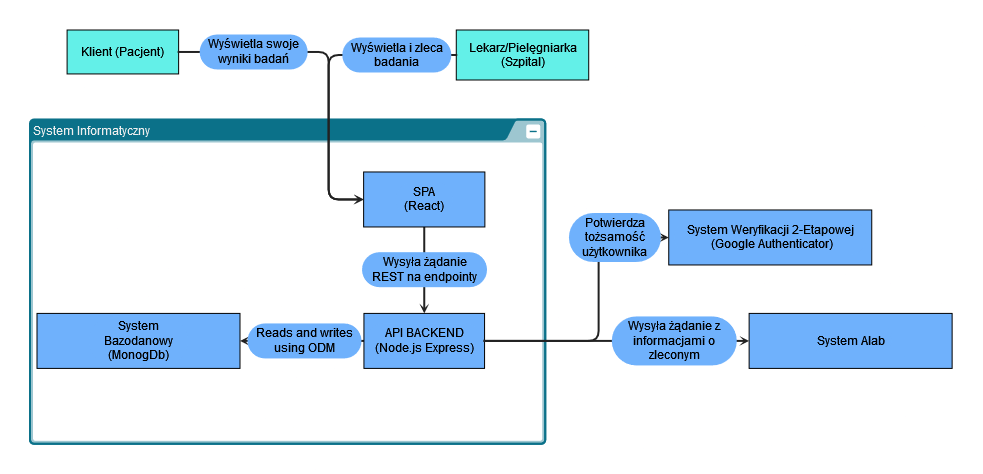
\includegraphics[width=0.8\textwidth]{Level_2_C4_Model.png}
    \caption{Schemat architektury\label{fig:arch}}
\end{figure}

Backend jest napisany w języku JavaScript z użyciem środowiska Node.js.
Aby zapewnić czytelność i łatwiejszy rozwój kod został podzielony na moduły w poszczególnych plikach.
Poniżej znajduje się lista modułów wraz z krótkim opisem.

\begin{itemize}
    \item \textbf{index.js} - główny plik aplikacji, zawiera konfigurację serwera, endpointów oraz uruchamia go.
    \item \textbf{auth.js} - moduł definiujący metody weryfikacyjne dla Passport.js.
    \item \textbf{controllers.js} - moduł zawierający kontrolery, czyli funkcje obsługujące zapytania HTTP.
    \item \textbf{db.js} - moduł odpowiedzialny za połączenie z bazą danych.
    \item \textbf{env.js} - moduł odpowiedzialny za wczytanie zmiennych środowiskowych.
    \item \textbf{models.js} - moduł zawierający modele danych.
\end{itemize}

Schemat zależności między modułami znajduje się na schemacie \ref{fig:dependency}.

\begin{figure}[h]
    \centering
    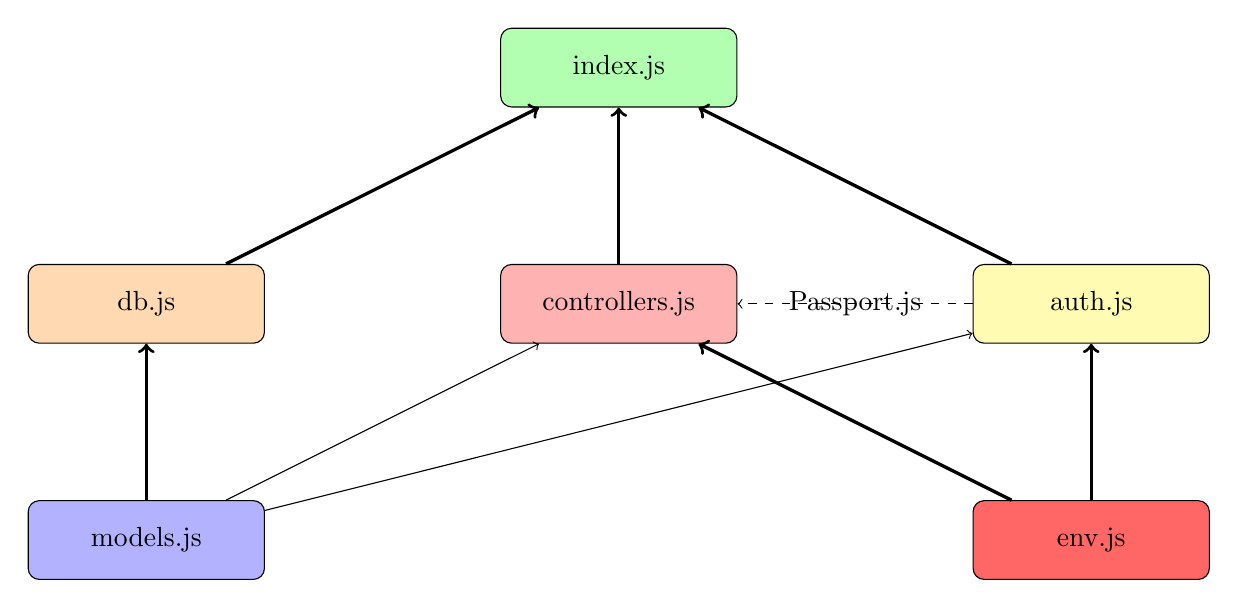
\begin{tikzpicture}[node distance=3cm]
        \node[module, fill=green!30] (index) {index.js};

        \node[module, fill=orange!30, below of=index, xshift=-6cm] (db) {db.js};
        \node[module, fill=blue!30, below of=db] (models) {models.js};
        
        \node[module, fill=red!30, below of=index, xshift=0] (controllers) {controllers.js};

        \node[module, fill=yellow!30, below of=index, xshift=6cm] (auth) {auth.js};
        \node[module, fill=red!60, below of=auth] (env) {env.js};

        
        \draw [->, very thick] (db) -- (index);
        \draw [->, very thick] (controllers) -- (index);
        \draw [->, very thick] (auth) -- (index);
        \draw [dashed, ->] (auth) -- node[anchor=center]{Passport.js} (controllers);
        \draw [->, very thick] (env) -- (auth);
        \draw [->, very thick] (env) -- (controllers);
        \draw [->, very thick] (models) -- (db);
        \draw [->] (models) -- (auth);
        \draw [->] (models) -- (controllers);

    \end{tikzpicture}
    \caption{Schemat wymagań\label{fig:dependency}}
\end{figure}

Trzeba zwrócić uwagę na nieoczywistą pośrednią zależność między modułami \codeword{auth.js} i \codeword{controllers.js}.
Rónież trzeba zauważyć różnice między przedstawionymi zależnościami.
Grubszymi strzałkami oznaczono pełny import modułu, a cieńszymi tylko import niektórych funkcji.

\indent Dokładniejszy schemat zależności między funkcjami, z perspektywy API znajduje się na schemacie \ref{fig:API}.
Przedstawiono na nim jakie funkcje są wywoływane podczas korzystania z API, oraz do którego pliku należą.

\begin{figure}[h]
    \centerfloat
    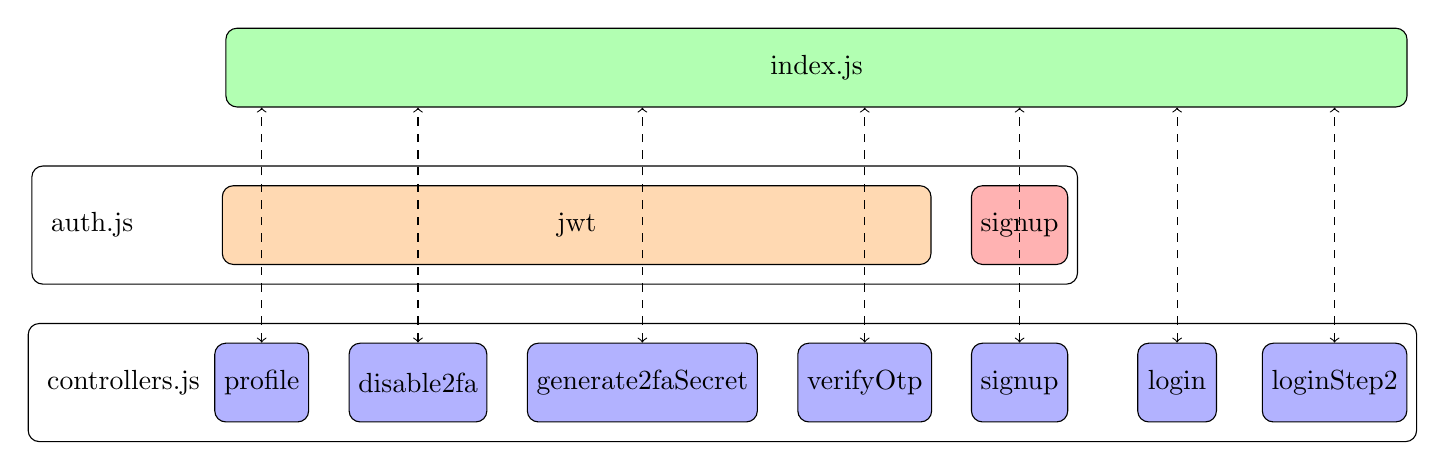
\begin{tikzpicture}[node distance=2cm, start chain=1 going right, start chain=2 going right]
        \tikzstyle{container} = [module, minimum height=1.5cm, minimum width=12cm]
        \tikzstyle{controller} = [module, minimum width=1cm, fill=blue!30]
        
        \node[module, fill=green!30, minimum width=15cm] (index) {index.js};
        
        \node[on chain=1, below of=index, xshift=-9.2cm] (authLabel) {auth.js};
        \node[module, fill=orange!30, minimum width=9cm, on chain=1, xshift=-1cm] (jwt) {jwt};
        \node[module, fill=red!30, minimum width=1cm, on chain=1, xshift=-1.5cm] (signup) {signup};
        \node[container, fit={(authLabel) (jwt) (signup)}] (authBox) {};

        \node[below of=authLabel, xshift=0.4cm] (containerLabel) {controllers.js};
        \node[controller, below of=jwt, xshift=-4cm, on chain=2] (profile) {profile};
        \node[controller, on chain=2, xshift=-1.5cm] (disable2fa) {disable2fa};
        \node[controller, on chain=2, xshift=-1.5cm] (generate2faSecret) {generate2faSecret};
        \node[controller, on chain=2, xshift=-1.5cm] (verifyOtp) {verifyOtp};
        \node[controller, below of=signup] (signupFunc) {signup};
        \node[controller, right of=signupFunc] (login) {login};
        \node[controller, right of=login] (loginStep2) {loginStep2};
        \node[container, fit={(profile) (signupFunc) (login) (loginStep2) (disable2fa) (generate2faSecret) (verifyOtp) (containerLabel)}] (components) {};

        \draw[<->, dashed] (profile) -- (profile|-index.south);
        \draw[<->, dashed] (disable2fa) -- (disable2fa|-index.south);
        \draw[<->, dashed] (generate2faSecret) -- (generate2faSecret|-index.south);
        \draw[<->, dashed] (verifyOtp) -- (verifyOtp|-index.south);
        \draw[<->, dashed] (signupFunc) -- (signupFunc|-index.south);
        \draw[<->, dashed] (login) -- (login|-index.south);
        \draw[<->, dashed] (loginStep2) -- (loginStep2|-index.south);

    \end{tikzpicture}
    \caption{Schemat architektury wewnętrznej API\label{fig:API}}
\end{figure}

\section{Baza danych}

Do projektu został wybrany silnik bazodanowy Mongoose.db.

\subsection{Schemat}

%TODO schemat bazy danych ERD? RM?

\subsection{Modele}

%TODO opis modeli jako klas

\end{document}